\documentclass[a4paper,8pt]{extarticle} % 使用更小的字号
\usepackage[top=0.4cm,bottom=0.4cm,left=0.4cm,right=0.4cm]{geometry} % 设置页边距
\usepackage{multicol} % 多栏排版
\usepackage{amsmath}
\usepackage{amssymb}
\usepackage{physics}
\usepackage{xcolor}
\usepackage[UTF8]{ctex} % Required for inserting images
\usepackage{longtable}
\usepackage{array}
\usepackage{tabularx}
\usepackage{graphicx}
\usepackage{float}
\usepackage{listings}
\usepackage[hidelinks]{hyperref}
\usepackage{titlesec}
\usepackage{tocloft}
\usepackage{parskip} % 用于段落格式控制

% 取消首行缩进
\setlength{\parindent}{0pt}
% 设置行距
\linespread{0.9}
% 设置公式间距
\setlength{\abovedisplayskip}{2pt}
\setlength{\belowdisplayskip}{2pt}
\setlength{\abovedisplayshortskip}{2pt}
\setlength{\belowdisplayshortskip}{2pt}

% 设置段落间距
\setlength{\parskip}{0.3ex}

% 定义蓝色、红色文本、背景色
\newcommand{\bluetext}[1]{\textcolor{blue}{#1}}
\newcommand{\redtext}[1]{\textcolor{red}{#1}}
\newcommand{\greentext}[1]{\textcolor{green}{#1}}
\newcommand{\yellowback}[1]{\colorbox{yellow}{#1}}

% 定义粗体
\newcommand{\black}[1]{\textbf{#1}}

% 优化多栏环境的分页设置
\raggedcolumns
\begin{document}
\begin{multicols}{3}
\setlength{\columnsep}{0.1cm} 

\redtext{定态微扰论}

\bluetext{微扰方程}:原方程:$(\hat{H}^{(0)} + \hat{H}')\psi_n = E_n\psi_n$;\\
零级方程:$\hat{H}^{(0)}\psi_n^{(0)} = E_n\psi_n^{(0)}$;\\
一级方程:$(\hat{H}^{(0)} - E_n^{(0)})\psi_n^{(1)} = -(\hat{H}' - E_n^{(1)})\psi_n^{(0)}$;\\
二级方程:$(\hat{H}^{(0)} - E_n^{(0)})\psi_n^{(2)} = -(\hat{H}' - E_n^{(1)})\psi_n^{(1)} + E_n^{(2)}\psi_n^{(0)}$。

\bluetext{无简并的微扰论}:能级一级修正:$E_n^{(1)} = H_{nn}' = \int \psi_n^{(0)*} \hat{H}'\psi_n^{(0)} \mathrm{d}\tau$;能级二级修正:$E_n^{(2)} = \sum_k \frac{|H_{kn}'|^2}{E_n^{(0)}-E_k^{(0)}}$;波函数一级修正:$\psi_n^{(1)}(x) = \sum_{k\neq n} \frac{H_{kn}'}{E_n^{(0)}-E_k^{(0)}} \psi_k^{(0)}(x)$。

\greentext{推导过程}
一级微扰推导:一级方程两边左乘 $\psi_n^{(0)*}$ 并积分:
$\langle\psi_n^{(0)}|(\hat{H}^{(0)}-E_n^{(0)})|\psi_n^{(1)}\rangle = -\langle\psi_n^{(0)}|(\hat{H}'-E_n^{(1)})|\psi_n^{(0)}\rangle$
得到:$0 = -(H'_{nn}-E_n^{(1)})$,$H'_{nn} $见上方,
因此 $E_n^{(1)} = H'_{nn}$

一级波函数推导:一级方程两边左乘 $\psi_k^{(0)*}$ 并积分:

由 $\int\psi_k^{(0)*}\psi_m^{(0)}(x)\mathrm{d}x=\delta_{km}$
对 $k\neq n$,得 $(E_n^{(0)}-E_k^{(0)})\langle\psi_k^{(0)}|\psi_n^{(1)}\rangle = \langle\psi_k^{(0)}|\hat{H}'|\psi_n^{(0)}\rangle = H'_{kn}$

$a_{nk}^{(1)} = \langle\psi_k^{(0)}|\psi_n^{(1)}\rangle = {H'_{kn}}/({E_n^{(0)}-E_k^{(0)}})$

代入 $\psi_n^{(1)} = \sum_m' a_{nm}^{(1)}\psi_m^{(0)}$

二级能级推导:一级波函数修正带入二级方程得到:
$(\hat{H}^{(0)} - E_n^{(0)})\psi_n^{(2)} = -\sum_m' \frac{H'_{mn}}{E_n^{(0)} - E_m^{(0)}} \hat{H}'\psi_m^{(0)} + E_n^{(1)}\sum_m' \frac{H'_{mn}}{E_n^{(0)} - E_m^{(0)}} \psi_m^{(0)} + E_n^{(2)}\psi_n^{(0)}$

利用正交性和左乘 $\psi_n^{(0)}$ 积分得到:
$0 = -\sum_m' \frac{H'_{mn}}{E_n^{(0)} - E_m^{(0)}} \int \psi_n^{(0)*} \hat{H}'\psi_m^{(0)} dt + E_n^{(2)}$

其中 $\int \psi_n^{(0)*} \hat{H}'\psi_m^{(0)} dt = H'_{nm}$
最终的二级微扰能量表达式:
$E_n^{(2)} = \sum_m' \frac{H'_{mn}H'_{nm}}{E_n^{(0)} - E_m^{(0)}}$
且$H'_{nm} = (H'_{mn})^*$

\bluetext{带有简并的微扰论}:

一级方程:$(\hat{H}^{(0)} - E_n^{(0)})\psi_{nl}^{(1)} = -(\hat{H}' - E_{nl}^{(1)})\psi_{nl}^{(0)}$;零级波函数:$\psi_{nl}^{(0)} = \sum_{j=1}^k c_{jl}^{(0)} \phi_{nj}^{(0)}$;一级波函数:$\psi_{nl}^{(1)} = \sum_m c_{ml}^{(1)}\phi_m^{(0)}$,其中 $c_{ml}^{(1)} = \frac{\int \phi_m^{(0)*} \hat{H}' \psi_{nl}^{(0)} \mathrm{d}\tau}{E_n^{(0)}-E_m^{(0)}}$;一级能级修正:$E_{nl}^{(1)}$ 为 $H'$ 对应子阵的本征值;二级能级修正:$E_{nl}^{(2)} = \sum_m \frac{|\int \phi_m^{(0)*} \hat{H}' \psi_{nl}^{(0)} \mathrm{d}\tau|^2}{E_n^{(0)}-E_m^{(0)}}$。

\bluetext{zeeman效应}:

实验证明,在外磁场中原子的能级会发生分裂。理论解释:电子的磁矩和外磁场有附加的相互作用能。$U_m = -\vec{M}\cdot\vec{B} = -M_z B = \frac{eB}{2\mu}(\hat{L}_z + 2\hat{S}_z)$,能量本征值改为:$E_{nlm_l m_s} = E_n + \frac{eB\hbar}{2\mu}(m_l + 2m_s)$,$(m_s = \pm\frac{1}{2})$。

\redtext{量子跃迁}

从一个能量本征态跃迁到另一个能量本征态,同时放出或吸收一定的能量。无扰动时无跃迁,有扰动时有跃迁。代入薛定谔方程:
$i\hbar\frac{\partial\Psi}{\partial t} = (\hat{H}_0 + \hat{H}'(t))\Psi(t)$

将 $\Psi$ 按 $\hat{H}_0$ 本质函数系 $\{\phi_n\}$ 展开,$\Psi(x,t) = \sum_n c_n(t)\phi_n(x)$,$|c_m(t)|^2$ 是 $|k\rangle \to |m\rangle$ 的跃迁几率。设 $c_n(t) = a_n(t)\exp\{-\frac{iE_n t}{\hbar}\}$,

带入得到
$i\hbar\sum_n \dot{a}_n(t)\exp(-\frac{iE_nt}{\hbar})\phi_n =$\\$ \sum_n a_n(t)\exp(-\frac{iE_nt}{\hbar})\hat{H}'(t)\phi_n$,
两边左乘$\phi_m^*$利用正交性 $\langle\phi_m|\phi_n\rangle = \delta_{mn}$ 得到严格方程:
$i\hbar\dot{a}_m(t) = \sum_n H'_{mn}(t)e^{i\omega_{mn}t}a_n(t)$

其中 $\omega_{mn} = \frac{1}{\hbar}(E_m - E_n)$ 为固有角频率。

\bluetext{含时间微扰法}:
系数展开:
$a_m(t) = a_m^{(0)} + a_m^{(1)}(t) + ...$
零级近似:
$i\hbar\frac{da_m^{(0)}}{dt} = 0 \Rightarrow a_m^{(0)}(t) = a_m^{(0)}(0)$

初始条件: $a_n^{(0)} = a_n^{(0)}(0) = \delta_{nk}$

一级近似:
$i\hbar\frac{da_m^{(1)}}{dt} = \sum_n H'_{mn}(t)e^{i\omega_{mn}t}a_n(0) = H'_{mk}(t')e^{i\omega_{mk}t}$
积分得:
对 $m \neq k$,$a_m(t) = a_m^{(1)}(t) = \frac{1}{i\hbar}\int_0^t H'_{mk}(t')e^{i\omega_{mk}t'} \mathrm{d}t'$,

跃迁几率(处于 $m$ 态的几率)为 $W_{k\to m} = |a_m(t)|^2$,跃迁速率为 $w = \frac{\mathrm{d}}{{\mathrm{d}t}}|a_m(t)|^2$ 决定了光谱线相对强度。
玻尔理论只能给出谱线频率

\bluetext{光驱动原子的电偶极跃迁}

$H' = e\vec{E}(t)\cdot\vec{x} = -e\vec{x}\cdot\vec{E}_0\sin(\omega t)$,$a_m(t) = a_m^{(1)}(t) =$ 

$ \frac{e\vec{x}_{mk}\cdot\vec{E}_0}{2\hbar}\left[\frac{e^{i(\omega_{mk}+\omega)t}-1}{i(\omega_{mk}+\omega)} - \frac{e^{i(\omega_{mk}-\omega)t}-1}{i(\omega_{mk}-\omega)}\right]$,共振条件为 $\omega_{mk} = \omega$ (吸收) 或 $\omega_{mk} = -\omega$ (受激辐射)。

\bluetext{选择定则}

$H'$矩阵元为零的跃迁被禁止,一般选择定则:$\hat{H}'_{mk}\neq 0$,电偶极选择定则:$\vec{x}_{mk}=\int{\psi_m^*(\vec{x})\vec{x}\psi_k(\vec{x}) d\tau} \neq 0$,
$|m\rangle$ 和 $|k\rangle$ 两态宇称相反,进一步考虑角动量选择准则得到$\Delta l = \pm1$,$\Delta m = 0, \pm1$;$\Delta m_s = 0$

微扰法成立的必要条件:$|a_m^{(1)}(t)|^2\ll 1$,尖锐共振$\omega_{mk}-\omega=0$且t足够大时微扰法失效,需要严格求解(Rabi震荡);微扰法对于通常的弱光在非共振情况一般是适用的。

\bluetext{Rabi震荡(非微扰理论)}

考虑较强的激光与原子共振或近共振
初始态条件:$a_1(0) = 1$;$a_2(0) = 0$,忽略非共振项:

由方程组:$i\frac{da_1}{dt} = \Omega a_2$,$i\frac{da_2}{dt} = \Omega^* a_1$,$\Omega = \frac{e\vec{E}_0\cdot\vec{x}_{12}}{2\hbar}$ 得到:$\frac{d^2a_1}{dt^2} = |\Omega|^2 a_1 = 0$ 解得:$a_1(t) = \cos(|\Omega|t)$,$a_2(t) = -i\frac{|\Omega|}{\Omega}\sin(|\Omega|t)$

对比微扰法,$i\frac{da_2}{dt} = \Omega^* a_1 \approx \Omega^* $,得到$a_2 = -i\Omega^* t$,非微扰退化为微扰的条件为:$|\Omega|t \ll 1$。

\bluetext{能量时间不确定关系}

定义某个力学量 $A$ 变化的特征时间为 $\tau \equiv \Delta A/|\frac{d\overline{A}}{dt}|$,

由 $\Delta A\Delta E \geq \frac{1}{2}|\overline{[A,H]}|$ 及 $\frac{d\overline{A}}{dt}=\frac{1}{i\hbar}\overline{[A,H]}$ 可以导出:
$\tau = \frac{\Delta A}{|\frac{d\overline{A}}{dt}|} = \frac{\Delta A}{\frac{1}{\hbar}|\overline{[A,H]}|} \geq \frac{\Delta A}{\frac{1}{\hbar}(2\Delta A\Delta E)} = \frac{\hbar}{2\Delta E}$

由此可得:$\Delta E \cdot \tau_A \geq \hbar/2$

\redtext{全同粒子}

微观粒子内部属性要么全同,要么显著不同,同一种粒子内部属性全同;量子力学中,在两个波包的重
叠区域不能区分2个全同粒子;全同粒子处于同一个环境中时,需要
考虑粒子的不可区别性(全同性)

典型例子:多电子原子中的电子、固体中的“公用”电子、原子核中的核子等

\bluetext{Bose 子与 Fermi 子}
交换任意两个粒子的全部坐标(空间坐标+自旋坐标),$\Psi(\cdots,q_i,\cdots,q_j,\cdots)=C\Psi(\cdots,q_j,\cdots,q_i,\cdots)$,交换对称 $(C=+1)$ 称为 Bose 子,交换反对称 $(C=-1)$ 称为 Fermi 子。Bose 子自旋 $s$ 为整数 (例如光子自旋 1、介子自旋 0),Fermi 子自旋 $s$ 为半整数 (例如电子、质子、中子自旋 1/2)。复合粒子取决于总自旋 (例如中性原子取决于中子数,偶为 Bose,奇为 Fermi)。

\bluetext{两个全同粒子系统}

分离变量形式特解 $\psi(q_1,q_2) = \psi_1(q_1)\psi_2(q_2)$ 不满足全同性要求,将其对称化(反对称化)处理:$\psi_{\pm}(q_1,q_2) = C[\psi_1(q_1)\psi_2(q_2) \pm \psi_1(q_2)\psi_2(q_1)]$,

\greentext{证明这个形式是唯一的}

(1) 设波函数:
$\psi(q_1,q_2) = c_1\psi_1(q_1)\psi_2(q_2) + c_2\psi_1(q_2)\psi_2(q_1)$

(2) 交换性质:
$\psi(q_2,q_1) = C\psi(q_1,q_2), (C = \pm1)$

(3) 代入求解:
$(c_1 - Cc_2)\psi_1(q_2)\psi_2(q_1) + (c_2 - Cc_1)\psi_1(q_1)\psi_2(q_2) = 0$
(4) 解得:
$c_2 = Cc_1 = \pm c_1$

(5) 最终形式:
$\psi(q_1,q_2) = C'[\psi_1(q_1)\psi_2(q_2) \pm \psi_1(q_2)\psi_2(q_1)]$

\bluetext{Pauli 不相容原理}

不可能有两个或更多的费米子处于完全相同的单粒子态中

重要体现,如
–元素周期表的物理根源(电子是费米子,每
个壳层能够容纳的电子数有限);
–固体中的能带填充(存在满带和不满带)
–电子束无法像激光那样输出
–中子星(存在简并压强)。

\greentext{Bose/Fermi 性质的不变性证明}

设含时薛定谔方程:
$i\hbar\frac{\partial\Psi}{\partial t} = H(q_1,q_2,...)\Psi(t,q_1,q_2,...)$

两个条件:
1) $H(q_2,q_1,...) = H(q_1,q_2,...)$
2) $\Psi(t,q_2,q_1,...) = C\Psi(t,q_1,q_2,...)$ $(C = \pm1)$

由此可得:
$\frac{\partial\Psi(t,q_2,q_1,...)}{\partial t} = C\frac{\partial\Psi(t,q_1,q_2,...)}{\partial t}$

时间演化:
$\Psi(t+dt,q_2,q_1,...) = \Psi(t,q_2,q_1,...) + \frac{\partial\Psi(t,q_2,q_1,...)}{\partial t}dt$
$= C\Psi(t,q_1,q_2,...) + C\frac{\partial\Psi(t,q_1,q_2,...)}{\partial t}dt$
$= C\Psi(t+dt,q_1,q_2,...)$

\bluetext{全同粒子的性质}

例子:一维无限深势阱中有两个电子TODO

一般含时间解由所有定态解叠加生成,自然也满足交换反对称性

例一:等效吸引和等效排斥作用

例二:两粒子占据两个正交单粒子态,有多少种可能情况

\redtext{混合态}

不能确切地知道状态波函数的情况下,只能借助于统计方法描述系统的状态,不是叠加态(叠加态有确定的波函数,混合态只能给出波函数的概率分布)。$\langle F \rangle = \sum_{\psi} P_{\psi}\langle F \rangle_{\psi} = \sum_{\psi} P_{\psi} \langle\psi| F |\psi\rangle$。

纯态例子 $|\psi\rangle=\sum_{n}c_n|\psi_n\rangle$

$\langle F \rangle=\langle\psi|F|\psi\rangle$
$=\sum_{mn}c_m^*c_n\langle\psi_m|F|\psi_n\rangle$
$=\sum_n|c_n|^2\langle\psi_n|F|\psi_n\rangle+\sum_{mn}^\prime c_m^*c_n\langle\psi_m|F|\psi_n\rangle$

\bluetext{密度算符}

纯态: $\rho \equiv |\psi\rangle \langle\psi|$,定义 $\operatorname{tr}(A) \equiv \sum_{n}\langle n|A|n\rangle$,则有 $\operatorname{tr}(F\rho) = \operatorname{tr}(\rho F) = \langle F \rangle$;混合态:$\rho \equiv \sum_{\psi} P_{\psi}|\psi\rangle \langle\psi|$,则有 $\langle F \rangle \equiv \operatorname{tr}(F\rho)$。运动学方程:$\frac{\mathrm{d}}{\mathrm{d}t}\rho = \frac{1}{i\hbar}[H,\rho]$。

\redtext{热力学公式}

- 热力学第零定律(热平衡原理)

- 热力学第一定律:闭系:$\mathrm{d}E = \overline{\mathrm{d}Q} + \overline{\mathrm{d}W} = \overline{\mathrm{d}Q} - P\mathrm{d}V$;开系:$\mathrm{d}E = \overline{\mathrm{d}W} + \overline{\mathrm{d}Q} + \sum_i \mu_i\mathrm{d}n_i$。

- 热容量:$C_V = \left(\frac{\partial E}{\partial T}\right)_V$,$C_P = \left(\frac{\partial H}{\partial T}\right)_P$,其中 $H = E + PV$。

- 热力学第二定律:$\mathrm{d}S \geq \frac{\overline{\mathrm{d}Q}}{T}$,可逆过程时取等号。Clausius 表述:不可能把热量从低温物体传到高温物体而不引起其他变化。Kelvin 表述:不可能从单一热源取得热量使之完全变成有用功而不引起其他变化。

- 热力学第三定律:不可能用有限次的步骤使系统的温度降低到绝对零度

- 热力学基本函数:$H = E + PV$,$F = E - TS$,$G = E + PV - TS$。

- 重要的微分式:$\mathrm{d}E = T\mathrm{d}S-P\mathrm{d}V$,$\mathrm{d}H = T\mathrm{d}S+V\mathrm{d}P$,$\mathrm{d}F = -S\mathrm{d}T-P\mathrm{d}V$,$\mathrm{d}G = -S\mathrm{d}T + V\mathrm{d}P$。

- 麦克斯关系:$\left(\frac{\partial T}{\partial V}\right)_S = -\left(\frac{\partial P}{\partial S}\right)_V$,$\left(\frac{\partial T}{\partial P}\right)_S = \left(\frac{\partial V}{\partial S}\right)_P$,$\left(\frac{\partial S}{\partial V}\right)_T = \left(\frac{\partial P}{\partial T}\right)_V$,$\left(\frac{\partial S}{\partial P}\right)_T = -\left(\frac{\partial V}{\partial T}\right)_P$。

- 理想气体熵变计算公式:$S(f) - S(i) = C_V \ln\left(\frac{T_f}{T_i}\right) + Nk\ln\left(\frac{V_f}{V_i}\right)$。

- 化学势:$\mu = \left(\frac{\partial E}{\partial N}\right)_{S,V} = \left(\frac{\partial H}{\partial N}\right)_{S,P} = \left(\frac{\partial F}{\partial N}\right)_{S,P} = \left(\frac{\partial F}{\partial N}\right)_{T,V} = \left(\frac{\partial G}{\partial N}\right)_{T,P}$。

- 热力学能量方程$dE(T,V) = \left(\frac{\partial E}{\partial T}\right)_V dT + \left(\frac{\partial E}{\partial V}\right)_T dV = C_v dT + \left(\frac{\partial E}{\partial V}\right)_T dV$
$C_P = \left(\frac{dQ}{dT}\right)_P =$ 

$ \left(\frac{dE + PdV}{dT}\right)_P = \left[\frac{C_v dT + \left(\frac{\partial E}{\partial V}\right)_T dV + PdV}{dT}\right]_P$

$= C_V + \left[P + \left(\frac{\partial E}{\partial V}\right)_T\right]\left(\frac{\partial V}{\partial T}\right)_P \Rightarrow \left(\frac{\partial E}{\partial V}\right)_T = (C_P - C_V)\left(\frac{\partial T}{\partial V}\right)_P - P$

$dE(T,V) = C_V dT + \left[(C_P - C_V)\left(\frac{\partial T}{\partial V}\right)_P - P\right]dV$

- 如果一个过程发生以后,我们有办法使它和它的外界同时回到
初始态,这个过程称为可逆过程。

- 可逆放热过程一定是熵减少的过程,自由绝热膨胀是不可逆过程,熵增加(构造可逆过程,$\Delta S=nRln(V_2/V_1)$)

- \greentext{证明可逆热机效率最高}:假设热机B比可逆热机A效率更高,则可利用B所做的功的一部分推动A逆向运行(另一部分功输出到外界),而最后2个热机的工作物质
和高温热源都没有变化,唯一变化是从单一(低温)热源吸取热量而全部变成了有用的功

- \greentext{证明热机效率等于温度之比}

$dQ = dE + PdV = C_v dT + PdV = 0$
$ dT = \frac{PdV + VdP}{nR}$
$\Rightarrow C_v \frac{PdV + VdP}{nR} + PdV = 0$ (1)

$C_p - C_v = nR$
$\gamma \equiv \frac{C_p}{C_v}$
$\Rightarrow nR = C_v(\gamma-1)$

$C_v \frac{PdV + VdP}{C_v(\gamma-1)} + PdV = 0 \rightarrow VdP + \gamma PdV = 0 \rightarrow \frac{dP}{P} + \gamma \frac{dV}{V} = 0$
$\Rightarrow PV^\gamma = const$ (绝热方程)

$(4 \rightarrow 1)$ $T_1V_1^{\gamma-1} = T_2V_4^{\gamma-1}$
$(2 \rightarrow 3)$ $T_1V_2^{\gamma-1} = T_2V_3^{\gamma-1}$
$\Rightarrow \frac{V_2}{V_1} = \frac{V_3}{V_4}$

$Q_1 = \int_1^2 PdV = \int_1^2 \frac{nRT_1}{V}dV = nRT_1 \ln(\frac{V_2}{V_1})$

$Q_2 = \int_3^4 PdV = -\int_3^4 \frac{nRT_2}{V}dV = nRT_2 \ln(\frac{V_3}{V_4})$

$\eta = \frac{W}{Q_1} = \frac{Q_1-Q_2}{Q_1} = 1-\frac{Q_2}{Q_1} = 1-\frac{T_2}{T_1}$

- \greentext{证明G(T,P,N)=Ng(T,P),即为化学势}
$dE = TdS - PdV + \mu dN$
$G = E + PV - TS$
$dG = -SdT + VdP + \mu dN$
$\mu = \left[\frac{\partial G}{\partial N}\right]_{T,P}$

\bluetext{Language乘子法}

粒子数($\sum_i n_i = N$)和能量($\sum_i n_i\varepsilon_i = E$),$F = \ln W\{n_i\} + \alpha(N-\sum_i n_i) + \beta(E-\sum_i n_i\varepsilon_i)$ 最可几分布。$\alpha(\mu,T) = -\frac{\mu}{kT}$,$\beta(T) = \frac{1}{kT}$。
\greentext{证明:构造两个有能量交换和(无)物质交换的系统}
$\ln W_B\{n_i\} \approx \sum_i [(n_i + g_i)\ln(n_i + g_i) - n_i \ln n_i - g_i \ln g_i]$
$\frac{\partial}{\partial n_i}\ln W_B\{n_i\} \approx \ln(\frac{g_i}{n_i} + 1)$,

$\ln W_F\{n_i\} \approx \sum_i [g_i \ln g_i - n_i \ln n_i - (g_i - n_i)\ln(g_i - n_i)]$
$\frac{\partial}{\partial n_i}\ln W_F\{n_i\} \approx \ln(\frac{g_i}{n_i} - 1)$,

进而由 $\frac{\partial F}{\partial n_i} = 0$ 有 $\ln(1 \pm \frac{g_i}{n_i}) - \alpha - \beta\varepsilon_i = 0$ 即得

\bluetext{四种统计}
$e^{\alpha+\beta\varepsilon_i} \gg 1 \Rightarrow e^\alpha \gg 1$满足能级非简并条件
等价于$n\lambda^3 \ll 1$,$\lambda = \frac{h}{p} = \frac{h}{\sqrt{2\pi mkT}}$
代入单原子理想气体$e^\alpha = \frac{z}{N}$即证明

满足可区分粒子或者$e^\alpha \gg 1$时,玻尔兹曼统计适用

\begin{figure}[H]
    \vspace{-0.3cm}
    \centering
    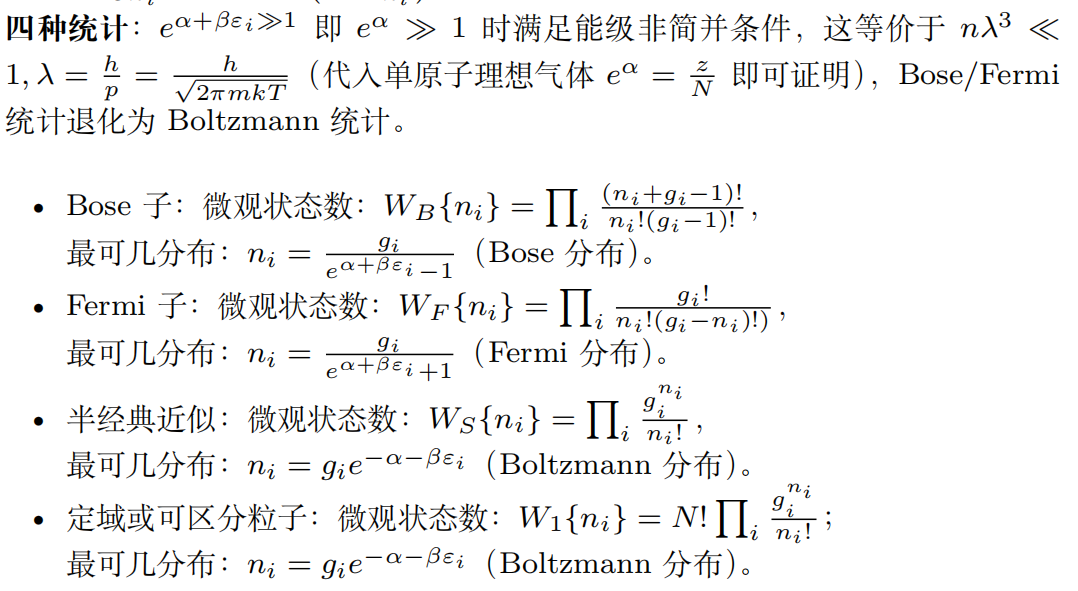
\includegraphics[width=0.33\textwidth]{images/1.png}
    \vspace{-0.6cm}
\end{figure}

\bluetext{配分函数}:定义配分函数$z=\sum_i g_i e^{-\beta\varepsilon_i}$

\begin{figure}[H]
    \vspace{-0.3cm}
    \centering
    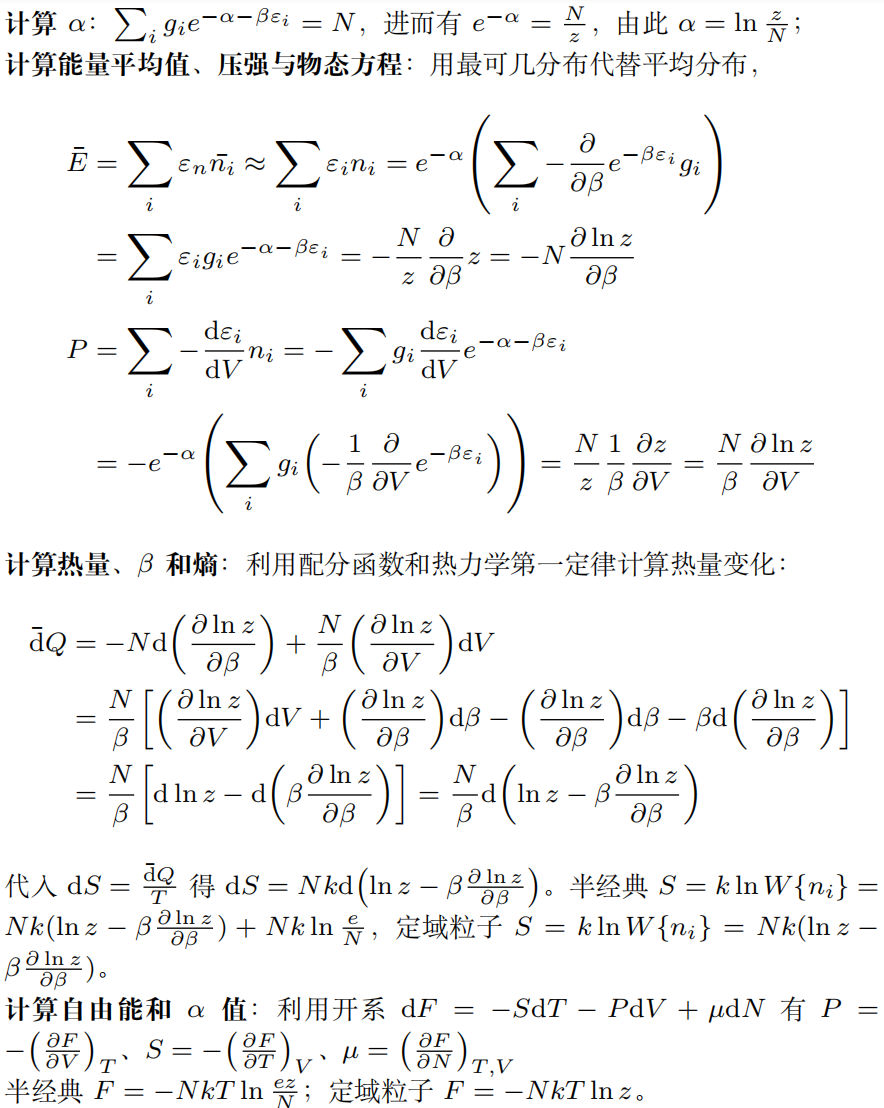
\includegraphics[width=0.33\textwidth]{images/2.png}
    \vspace{-0.6cm}
\end{figure}

\bluetext{典型例子}:立方体容器中的气体
$\varepsilon_i = $

$\frac{\hbar^2}{2m}\left[\left(\frac{n_x\pi}{L}\right)^2 + \left(\frac{n_y\pi}{L}\right)^2 + \left(\frac{n_z\pi}{L}\right)^2\right] = A_iV^{-2/3}$

$\frac{d\varepsilon_i}{dV} = -\frac{2}{3}A_iV^{-2/3-1} = -\frac{2}{3}\frac{\varepsilon_i}{V}$

$P = \sum_i -\frac{d\varepsilon_i}{dV}n_i = \frac{2}{3V}\sum_i\varepsilon_in_i = \frac{2}{3}\frac{\bar{E}}{V}$

\greentext{证明k是玻尔兹曼常数}

由于$\beta$是$dQ$的积分因子, 设$\beta dQ = dS'$ (1)

根据热力学, $dQ = TdS$, 代入(1)得:
$dS' = \beta TdS$

因$\beta = \beta(T)$, 可设$S' = S'(S,T)$,

于是$dS' = \frac{\partial S'}{\partial S}dS + \frac{\partial S'}{\partial T}dT$

得到$\beta T = \frac{\partial S'}{\partial S}$ (4)
$\frac{\partial S'}{\partial T} = 0$

设$S' = S'(S)$, $\frac{\partial S'}{\partial S} = f(S)$, 代入(4)得

$\beta(T)T = f(S) =$ 常数 $(设为\frac{1}{k})$ $\rightarrow$ $\beta = \frac{1}{kT}$

\bluetext{熵}:$\mathrm{d}S = k\mathrm{d}(\ln W_{sm}\{n_i\})$,$S = k\ln W_s\{n_i\}$

\greentext{推导过程}:先有 $\overline{\mathrm{d}Q} = \frac{N}{\beta}\mathrm{d}(\ln z - \beta\frac{\partial\ln z}{\partial\beta})$,再根据 

$\ln W_{sm}\{n_i\} = \sum_i (n_i\ln g_i - \ln n_i!)|_{n_i=g_i\exp\{-\alpha-\beta\varepsilon_i\}} \approx \sum_i [n_i\ln g_i - n_i(\ln n_i-1)] \approx \sum_i [n_i\ln \frac{g_i}{n_i} + n_i]|_{\frac{g_i}{n_i}=\exp\{\alpha+\beta\varepsilon_i\}} = \sum_i n_i(\alpha + \beta\varepsilon_i + 1) = N\alpha + \beta E + N = N(\ln z - \beta\frac{\partial\ln z}{\partial\beta}) + N(1-\ln N)$,两边乘 $k$ 对比即得。

\bluetext{量子态的相体积}: 在能量准连续的条件下,对于量子数足够大的状态,一个量子态在 $\mu$ 空间中对应 $h^r$ 的相体积,$r$ 是粒子的自由度数。能级准连续近似成立的条件为 $\frac{\Delta \varepsilon_i}{kT} \ll 1$。

\bluetext{态密度}: 相空间中能量曲面 $\varepsilon$ 包围体积为 $\Omega(\varepsilon)$,则 $\varepsilon$ 到 $\varepsilon + \mathrm{d}\varepsilon$ 能量间隔内量子态数目是 $g(\varepsilon)\mathrm{d}\varepsilon = \frac{\mathrm{d}\Omega(\varepsilon)}{h^r}J$,$J$ 是内部简并度,基本粒子为自旋简并度。

\bluetext{理想气体}: 近独立粒子组成、符合半经典分布,能级准连续情况下有: $n(\varepsilon)\mathrm{d}\varepsilon = g(\varepsilon)e^{-\alpha-\beta\varepsilon}\mathrm{d}\varepsilon$。对于 $n$ 维单原子理想气体有: $z(\beta,V) = \int_0^{\infty}e^{-\beta\varepsilon}g(\varepsilon)\mathrm{d}\varepsilon = \frac{V}{h^n}\left(\frac{2\pi m}{\beta}\right)^{n/2}$。

\bluetext{相空间算配分函数}: $\varepsilon = \frac{p_x^2}{2m} + \frac{p_y^2}{2m} + \frac{p_z^2}{2m} + U(x,y,z)$, $z(\beta,V) = \frac{1}{h^3}\left(\frac{2\pi m}{\beta}\right)^{3/2}\cdot\int e^{-\beta U(x,y,z)}\mathrm{d}x\mathrm{d}y\mathrm{d}z$

\bluetext{Boltzmann统计模型}

\textbf{三维单原子非相对论气体}:$\varepsilon = p^2/2m$,

势阱模型:$\varepsilon_i = \frac{h^2}{8mL^2}(n_1^2+n_2^2+n_3^2)$
$\Omega(\varepsilon) = \frac{4\pi V}{3}(2m\varepsilon)^{3/2}$,$g(\varepsilon)d\varepsilon = J\frac{2\pi V(2m)^{3/2}}{h^3}\sqrt{\varepsilon}d\varepsilon$,

$z(\beta,V)=\frac{V}{h^3}\left(\frac{2\pi m}{\beta}\right)^{3/2}$,

$lnz=\frac{3}{2}\ln \frac{2\pi m}{h^2} - \frac{3}{2}\ln\beta + \ln V$

$E=-N\frac{\partial \ln z}{\partial \beta} = \frac{3}{2}\frac{N}{\beta} = \frac{3}{2}NkT$

$P=\frac{N}{\beta}\frac{\partial \ln z}{\partial V} = \frac{NkT}{V}$

$F(T,V) = -NkT(\frac{3}{2}\ln kT + \ln \frac{V}{N} + \frac{3}{2}\ln \frac{2\pi m}{h^2} + 1)$

$S(T,V) = Nk(\frac{3}{2}\ln kT + \ln \frac{V}{N} + j + \frac{5}{2})$,$j = \frac{3}{2}\ln \frac{2\pi m}{h^2}$
$\mu = kT(\ln \frac{N}{V} - \frac{3}{2}\ln kT - j)$

\textbf{三维单原子光子气体}:
$\varepsilon = cp$,势阱模型:$\varepsilon_i = \frac{hc}{2L}\sqrt{n_1^2+n_2^2+n_3^2}$,$C_V = 3Nk$
$\Omega(\varepsilon) = \frac{4\pi V}{3c^3}\varepsilon^3$,$g(\varepsilon)d\varepsilon = J\frac{4\pi V}{(hc)^3}\varepsilon^2d\varepsilon$

\textbf{三维双原子非相对论气体}:
$C_V = C_V^t + C_V^r + C_V^v$(平动、转动、振动),其中 $C_V^t = \frac{3}{2}Nk$,$C_V^r = Nk$,$C_V^\nu = Nk\frac{x^2e^x}{(e^x-1)^2} \ll Nk$

转动:$\Omega^r(\varepsilon^r) = 8\pi^2I\varepsilon^r$,$g^r(\varepsilon^r)d\varepsilon^r = \frac{8\pi^2I}{h^2}d\varepsilon^r$,$z^r(\beta) = \frac{8\pi^2I}{h^2}\frac{1}{\beta}$
$\varepsilon_0^r = \frac{h^2}{8\pi^2I}$,特征温度为$\theta^r=\varepsilon_0^r/k$,准连续条件变为$\theta^r \ll T$

振动:谐振子能级$\varepsilon=(n+1/2)h\nu$,$\theta^\nu = \frac{h\nu}{k}$,$T \ll \theta^\nu$

整体:$\Omega(\varepsilon) = \frac{64}{15}\pi^3VI(2m)^{3/2}\varepsilon^{5/2}$,$g(\varepsilon)d\varepsilon = \frac{32\pi^3VI(2m)^{3/2}}{3h^5}\varepsilon^{3/2}d\varepsilon$

\textbf{二维单原子非相对论气体}:
$C_v = Nk$,$\Omega(\varepsilon) = 2\pi mS\varepsilon$,$g(\varepsilon)d\varepsilon = \frac{2\pi mS}{h^2}d\varepsilon$

\textbf{Einstein晶格振动模型}:
$H = \sum_{i=1}^{3N}(\frac{1}{2m}p_i^2 + \frac{m}{2}(2\pi\nu_i)^2q_i^2)$,假设3N个振动模式固有频率都相等 $\nu_i = \nu$,$\varepsilon = \varepsilon_n = (n+\frac{1}{2})h\nu$
$z(\beta) = \frac{e^{-1/2\beta h\nu}}{1-e^{-\beta h\nu}}$,$\overline{E}(T) = 3Nh\nu(\frac{1}{2} + \frac{1}{e^{\beta h\nu}-1})$,$C_\nu = 3Nk\varepsilon(\beta h\nu)$,其中
$\varepsilon(x) = \frac{x^2e^x}{(e^x-1)^2}$ 称为Einstein函数,$S = 3Nk[\frac{\beta h\nu}{e^{\beta h\nu}} - \ln(1-e^{-\beta h\nu})]$

令$\theta_E = \frac{h\nu}{k}(100K-300K)$,称为Einstein温度;

(1)高温时,$T \gg \theta_E, x=\theta_E/T \ll 1, C_\nu \approx 3Nk$;

(2)低温时,$C_\nu \approx 3Nk(\frac{\theta_E}{T})^2e^{-\theta_E/T}$

\bluetext{Bose/Fermi 统计公式}: 上Bose, 下Fermi,

$\ln W\{n_i\} = \sum_i \left[n_i\ln\left(\frac{g_i}{n_i} \pm 1 \right) \pm g_i\ln\left(1 \pm \frac{n_i}{g_i}\right)\right]$,
$\Phi(\alpha,\beta,V) = \mp \sum_i g_i\ln\left(1 \mp e^{-\alpha-\beta\varepsilon_i}\right)$,

$N = -\frac{\partial\Phi}{\partial\alpha}$, $E = -\frac{\partial\Phi}{\partial\beta}$, $P = \frac{1}{\beta}\frac{\partial\Phi}{\partial V}$, $S = k\left(\Phi - \alpha\frac{\partial\Phi}{\partial\alpha} - \beta\frac{\partial\Phi}{\partial\beta}\right)$。

\bluetext{玻色-爱因斯坦凝聚 (BEC)}: Bose 气体在低于某临界温度时,气体中大部分粒子凝聚在最低能级。其化学势 $\mu < 0$,$T$ 越小化学势越高,越接近于 $0-$。临界温度: $T_c = \frac{h^2}{2\pi mk}\left(\frac{n}{2.612}\right)^{2/3}$ 即 $n\lambda^3(T=T_c) = 2.612$,$\lambda = \frac{h}{p} = \frac{h}{\sqrt{2\pi mkT}}$。

$N = \int_0^{\infty}\frac{g(\varepsilon)d\varepsilon}{e^{\varepsilon/kT_c}-1} = \frac{2\pi V(2m)^{3/2}}{h^3}\int_0^{\infty}\frac{\sqrt{\varepsilon}d\varepsilon}{e^{\varepsilon/kT_c}-1}=$

$\frac{2\pi V}{h^3}(2mkT_c)^{3/2}\int_0^{\infty}\frac{\sqrt{x}dx}{e^x-1} = 2.612V\left(\frac{2\pi mkT_c}{h^2}\right)^{3/2}$

即可解出临界温度。

\textbf{半经典极限条件}$e^{\alpha} \gg 1$,即$e^\alpha = z/N =(\frac{V}{N})(\frac{2m\pi kT}{h^2})^{3/2} \gg 1$,可以改写为$n\lambda^3 \ll 1$,

\textbf{比较}:另一种半经典近似条件——能级准连续条件

考虑平动能级:
$\varepsilon_i = \frac{h^2}{8mL^2}(n_1^2 + n_2^2 + n_3^2)$,$\Delta\varepsilon \approx \frac{h^2}{8mL^2}$
准连续条件 $\Delta\varepsilon \ll kT$ 要求 $\frac{h^2}{8mL^2} \ll kT$

即 $\frac{h^2}{8mL^2} \ll \frac{h^2}{2m\pi\lambda^2}$,即 $L \gg \frac{\sqrt{\pi}}{2}\lambda$

作为估算,可取 $L \gg \lambda$ ($\lambda = \frac{h}{\sqrt{2m\pi kT}}$)

\bluetext{光子气体}: (bose-einstein分布)腔内场域腔壁不断作用达到热平衡态,温度为 $T$。光子静止质量为零,能量和动量满足 $\varepsilon = cp$,$J = 2$。光子数不守恒!

$n_i = \frac{g_i}{e^{\beta\varepsilon_i}-1}$,$g(\nu)d\nu = \frac{4\pi JV}{c^3}\nu^2d\nu$,$n(\nu)d\nu = \frac{4\pi JV}{c^3}\frac{\nu^2}{e^{h\nu/kT}-1}d\nu$,
Planck 公式: $\bar{E}(\nu,T)d\nu = h\nu n(\nu)d\nu = \frac{8\pi V}{c^3}\frac{h\nu^3}{e^{h\nu/kT}-1}d\nu$,

\textbf{两个极限频率}
$h\nu/kT \ll 1$: $\bar{E}(\nu,T) \approx \frac{8\pi V}{c^3}kT\nu^2$(瑞利金斯公式),
$h\nu/kT \gg 1$: $\bar{E}(\nu,T) \approx \frac{8\pi V}{c^3}h\nu^3e^{-h\nu/kT}$(维恩公式),

总光子数: $N=\int_0^{\infty}n(\nu)d\nu=8\pi V \times 2.404\left(\frac{kT}{hc}\right)^3$,
总能量: $\bar{E} = bVT^4$,总能量密度: $u = \frac{\bar{E}}{V} = bT^4$,总面辐射强度: $J = \frac{1}{4}cu = \sigma T^4$,其中 $b = \frac{8\pi^5k^4}{15(hc)^3}$、$\sigma = \frac{2\pi^5k^4}{15h^3c^2}$。

% 也可以用振子模型TODO,体现了光的波粒二象性

\bluetext{声子气体}:声子不断产生和消灭,能量和动量满足: $\varepsilon = vp$,横波 $J = 2$,纵波 $J = 1$。
总声子数不守恒!根据总模式数只有 $3N$ 个, $\int_0^{\nu_D} g(\nu)d\nu = 3N$ 可以得到德拜频率。特征温度 $\theta_D = \frac{h\nu_D}{k}$,平衡态平均声子数$\bar{n_i} = \frac{g_i}{e^{h\nu_i/kT}-1}$。$n(\nu)d\nu = \frac{g(\nu)d\nu}{e^{\beta h\nu}-1}$,

本征模式:指具有有确定的频率、波矢、振动方向的特殊声波;• 引入声子概念后晶格的振动就被看做是声子气体的运动

de Broglie关系:
$\varepsilon = h\nu$
$\vec{p} = \hbar\vec{k}$ $(p = \frac{h}{\lambda})$
$\nu = \mathrm{v}/\lambda$
$\varepsilon = h(\mathrm{v}/\lambda) = \mathrm{v}(h/\lambda)$
$\Rightarrow \varepsilon = \mathrm{v}p$ (声子能量-动量关系)

Debye假设:频率有上限

\textbf{一维:}
$g(\nu)d\nu = 2L(\frac{2}{\mathrm{v_t}} + \frac{1}{\mathrm{v_l}})d\nu = B_1d\nu = \frac{3N}{\nu_D}d\nu$,$(0 \leq \nu \leq \nu_D)$
$n(\nu)d\nu = \frac{3N}{\nu_D}\frac{1}{e^{\beta h\nu}-1}d\nu$,$(0 \leq \nu \leq \nu_D)$,$\nu_D = \frac{3N}{B_1}$
$\overline{E}(T,V) = \frac{3N}{\nu_D}\frac{(kT)^2}{h}\frac{\pi^2}{6}$,$C_V = Nk\pi^2\frac{T}{\theta_D}$

\textbf{二维:}
$g(\nu)d\nu = 2\pi S(\frac{2}{\mathrm{v}_t^2} + \frac{1}{\mathrm{v}_l^2})\nu d\nu = B_2\nu d\nu = \frac{6N}{\nu_D^2}\nu d\nu$, $(0 \leq \nu \leq \nu_D)$
$n(\nu)d\nu = \frac{6N}{\nu_D^2}\nu d\nu\frac{1}{e^{\beta h\nu}-1}$, $(0 \leq \nu \leq \nu_D)$, $\nu_D = (\frac{6N}{B_2})^{\frac{1}{2}}$
$\overline{E}(T,V) = \frac{6N}{\nu_D^2}(\frac{kT}{h^2})^3\cdot2.404$, $C_V = 18Nk(\frac{T}{\theta_D})^2\cdot2.404$

\textbf{三维:}
$g(\nu)d\nu = 4\pi V(\frac{2}{\mathrm{v}_t^3} + \frac{1}{\mathrm{v}_l^3})\nu^2d\nu = B_3\nu^2d\nu = \frac{9N}{\nu_D^3}\nu^2d\nu$, $(0 \leq \nu \leq \nu_D)$

$n(\nu)d\nu = \frac{9N}{\nu_D^3}\nu^2d\nu\frac{1}{e^{\beta h\nu}-1}$, $(0 \leq \nu \leq \nu_D)$, 

$\nu_D = (\frac{9N}{B_3})^{\frac{1}{3}}$合理性检验:取$v_t=v_l=v$,$\lambda_D = \frac{v}{\nu_D}=(\frac{4\pi V}{3N})^{1/3}$

$\overline{E}(T,V) = \frac{9N}{\nu_D^3}\int_0^{\nu_D}\frac{h\nu^3}{e^{\beta h\nu}-1}d\nu = \frac{9N}{y^3}kT\int_0^y\frac{x^3}{e^x-1}dx$, 
其中$y = \frac{h\nu_D}{kT}$,$x = \beta h\nu =\frac{h\nu}{kT}$

高温时:$y \ll 1$,$\overline{E}(T,V) = 3NkT$,$C_V = 3Nk$
% $C_V = 9Nk(\frac{kT}{h\nu_D})^3\int_0^y x^2\varepsilon(x)dx$, $y = \frac{h\nu_D}{kT}$

低温时: $y \gg 1$, $C_V = 3Nk\frac{4\pi^4}{5}(\frac{T}{\theta_D})^3$,其中$\theta_D = \frac{h\nu_D}{k}$,约为几百K

\bluetext{Fermi 气体}: 以电子气体为例,$J = 2$,计算 Fermi 能级时利用 $T \to 0$ 时 $\mu_0 = \varepsilon_F$,$N = \int_0^{\mu_0}g(\varepsilon)d\varepsilon$,$\bar{E_0} = \int_0^{\mu_0}\varepsilon g(\varepsilon)d\varepsilon$。

\textbf{零温情形}
T=0K的情形称为完全简并的电子Fermi气体。粒子从最低单粒子态填起,依次填充,直到填满为止(最高的单粒子能级叫做费米能级)
定义单个量子态上的平均粒子数$f_i=n_i/g_i$, $\alpha+\beta \varepsilon_i=(\varepsilon_i-\mu_0)/kT$

$f_i = \frac{1}{e^{\alpha+\beta\varepsilon_i}+1} = \left\{\begin{array}{ll}1, & \varepsilon_i < \mu_0\\0, & \varepsilon_i > \mu_0\end{array}\right.$

$g(\varepsilon) = J\frac{2\pi V(2m)^{3/2}}{h^3}\sqrt{\varepsilon}=CV\sqrt{\varepsilon}$,其中$J = 2$,$C = \frac{2\pi J(2m)^{3/2}}{h^3}$
$N = \sum_i n_i = \sum_{i(\varepsilon_i<\mu_0)} g_i = \int_0^{\mu_0} g(\varepsilon)d\varepsilon$
$=CV\int_0^{\mu_0} \sqrt{\varepsilon}d\varepsilon = \frac{2}{3}CV\mu_0^{3/2}$

电子 $\varepsilon_F = \mu_0 = (\frac{3N}{2CV})^{2/3} = \frac{h^2}{2m}(\frac{3}{8\pi}\frac{N}{V})^{2/3} \sim 10^{-18}-10^{-19}J$

$\bar{E_0} = \frac{2}{5}CV\mu_0^{5/2}$,单粒子平均能量$\frac{\bar{E_0}}{N} = \frac{3}{5}\mu_0$

$\bar{P_0} = \frac{2}{3}\frac{\bar{E_0}}{V} = \frac{2}{5}\frac{N\mu_0}{V}$,

\greentext{证明:以立方体容器为例}
$\varepsilon_i = \frac{(\hbar k)^2}{2m} = \frac{h^2}{2m}[(\frac{n_x\pi}{L})^2 + (\frac{n_y\pi}{L})^2 + (\frac{n_z\pi}{L})^2] = A_iV^{-2/3}$

$\frac{d\varepsilon_i}{dV} = -\frac{2}{3}A_iV^{-2/3-1} = -\frac{2}{3}\frac{\varepsilon_i}{V}$

$P = \sum_i -\frac{d\varepsilon_i}{dV}n_i = \frac{2}{3V}\sum_i\varepsilon_in_i = \frac{2}{3}\frac{\overline{E}}{V}$ ($\overline{E} = \sum_i n_i\varepsilon_i$)

\textbf{有限温度情形}(kT有限大但远小于$\mu_0$)

定义费米温度$T_F = \frac{\mu_0}{k}$,
$C_V = \frac{\pi^2}{2}Nk\left(\frac{kT}{\mu_0}\right) = \frac{\pi^2}{2}Nk\left(\frac{T}{T_F}\right)$,
近似解法: $\Delta\bar{E} \approx N\cdot\frac{kT}{\mu_0}\cdot 2kT$,$C_V = 4Nk\left(\frac{T}{T_F}\right)$。

相对论情况:

$n_i = \frac{g_i}{e^{\alpha+\beta\varepsilon_i}+1}$,$g(\varepsilon) = J\frac{4\pi V}{(hc)^3}\varepsilon^2$,

$\varepsilon_F = hc\left(\frac{3N}{4\pi JV}\right)^{\frac{1}{3}}$,
$N = \frac{4\pi JV}{3(hc)^3}\varepsilon_F^3$,$\bar{E_0} = \frac{3}{4}N\varepsilon_F$,$\bar{P_0} = \frac{1}{3}\frac{\bar{E_0}}{V}$。
\end{multicols}
\end{document}